\chapter{Solution}
\label{ch:solution}
%Approx. 10 pages


\section{Implementation}

\subsection{Graph}
The ship was modelled out as a graph with nodes and connections. There was used two different types of graph when testing, one which was created manually and one that was randomly made each time. The nodes themselves represented a room on board the ship and the connections from that room to another room, so that you could go from one room to another and back again. The nodes could hold some different parameters as if they were an exit so the passengers could get to safety or if they were lethal. In this project we only used 1 or 0, where 1 was 100\% chance of death and 0 was 0\%, however we had implemented it so it was possible to set other chances. The reason for only choosing to have 0 or 1 during the testing, was to keep it simple, otherwise we might get overwhelmed in to many parameters that might impact the results. 
\begin{wrapfigure}{r}{10cm} % "placement and width parameter for the width of the image space.
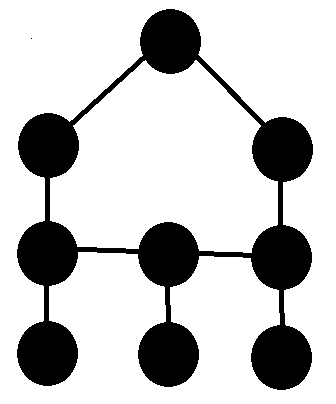
\includegraphics[width=40mm]{manuallyGraph.png}
\caption{Graph with 8 nodes, where 2 are lethal and there is 1 exit.}
\label{smalgraph}
\end{wrapfigure}

\subsection{Brute force}
The main algorithms that was used to find its way through the graph was a brute force, random and Ant Colony optimization. Brute force was the first algorithm to run, it went trough all the nodes going one step at the time and finding all the possible solutions for that node. When it was done it picked the shortest solution with the least likely hood of dying and set that as that nodes best route, then to the next node doing the same. Also if we used randomly generated graph, it checked if a human was in a node that had a possible way to an exit, if not it was updated so the human would not walk forever in random. 

\subsection{Random}
Random was simple in it's way that each human took one step and checked if they had reached an exit or died in that node. If the human started in a node that could not reach an exit node, it was counted as a dead human as it could not get to safety. In real situations, the possibility of people getting stuck like this is unlikely, however it might happen if parts of the ship collapses.

\subsection{Ant Colony Optimization}
In our Ant Colony algorithm, it started out the same way as random, by walking through the graph to find an exit. Once if do find an exit, it reports back in each node it visited and adds pheromones based on how long the path was and how lethal it was. Since we only used 1 and 0 in this situation, it would only increase the pheromones when there was no lethal nodes. Then it does the same again, walk around a bit less randomly, as the pheromones gives a higher chance of choosing the same path as the previous one. After some turns a path will develop as the AntSystem walks through the graph from an node to the exit.

%\section{Proposed solution / algorithm}

%\subsection{The basic algorithm}

%\subsection{Discussion of design issues}


%\subsection{Algorithmic Enhancements}


%\subsection{Discussion of the Parameter Space}


%\section{Prototype}

%\section{Justification of Claim to Originality}

%\section{Valuation of Contribution}

%\section{Alternatives}
